 In this chapter, we explore the related work of virtualized TAS. We first outline recent 
 works on TCP acceleration (section 3.1), then we list the state-of-the-art methods for network virtualization (section 3.2).



\section{TCP acceleration techniques}


\section{Network Virtualization}
Public cloud providers, such as Amazon Web Services (AWS), Microsoft Azure, 
and Google Cloud Platform (GCP), have taken different approaches to network 
virtualization for their customers. While Microsoft has been following a 
hardware-assisted procedure to provision networking demands, Google has been 
utilizing a software-only approach. Section 3.2.1 elaborates on network 
virtualization using a pure software technique, and section 3.2.2 explores 
hardware-assisted network virtualization.


\subsection{Network Virtualization in Software}


\subsubsection{Google Snap system for host networking}

As one of the primary cloud providers with internet-based products 
that are used by a wide range of users, Google has prioritized 
the following three main needs for host networking in their data centers. 

\begin{enumerate}
    \item The network bandwidth is continuously increasing and delivering 
    novel approaches for edge switching and bandwidth management 
    is essential. Therefore they require a system that enables 
    fast delivery of innovative paradigms.
    \item Rich virtualization features must be provided on top of 
    host networking to enable cloud computing.
    \item Distributed data-intensive applications require low latency 
    and high throughput for their communication. As a consequence, the 
    host networking system should be optimized with regard to these applications.
\end{enumerate}

Using kernel for networking at the end-hosts does not align with these 
requirements and has the following three primary drawbacks for 
cloud providers such as Google.

\begin{enumerate}
    \item Developing new features takes more effort 
    when host networking is done on the kernel side, and 
    fewer developers have the desired expertise in kernel development.
    This makes the delivery of new paradigms harder and more expensive.

    \item Only a subset of upgrades could be applied by probing new 
    modules to the kernel  and main upgrades require the system reboot 
    which comes with the high cost of application migration. 
    
    \item Upstream updates from the Linux community try to optimize for 
    general case and may have conflicts with the vertical optimization
    applied for distributed data-intensive applications.
\end{enumerate}

To reach the requirements of data-center networking and to mitigate the 
drawbacks of using kernel in development of end-host network stack, 
Google has proposed Snap. Snap is a userspace networking system, which is 
initially inspired from microkernel architecture. By residing on the  
userspace, the development of new features has became faster and 
upgrades to networking stack can be applied transparently. Moreover, in 
comparison to Linux Kernel networking stack it provides higher throughput.

\begin{figure}
\small
\center
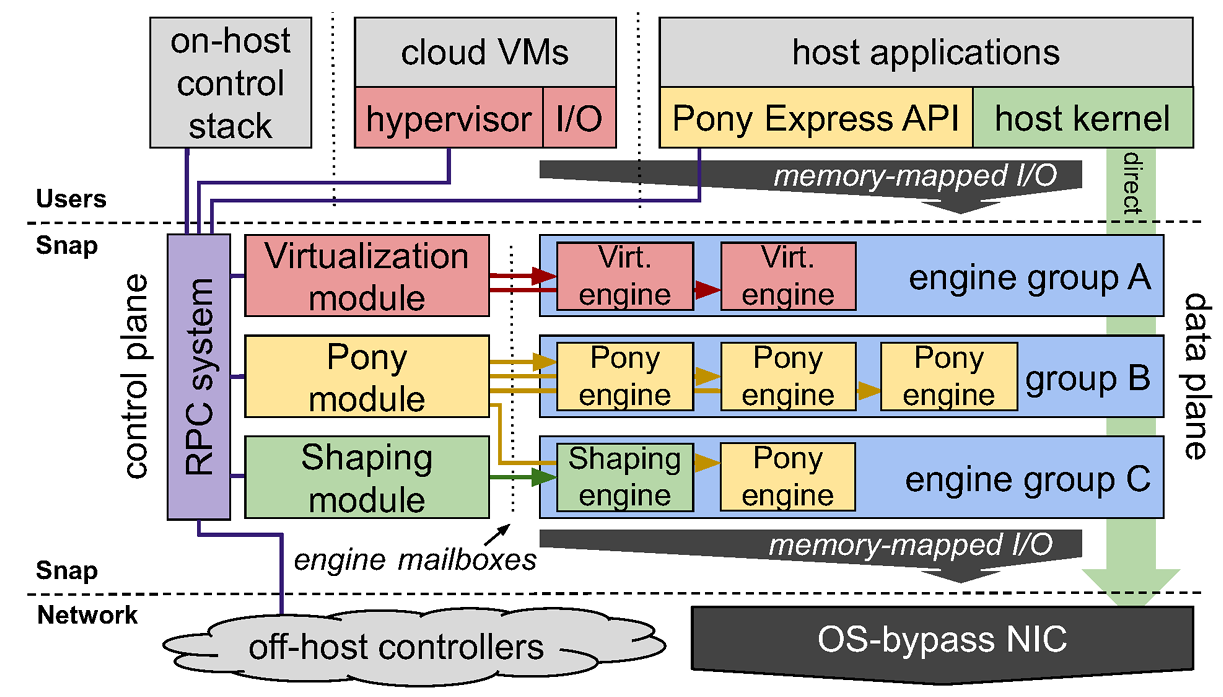
\includegraphics[width=\textwidth]{../Figures/snap.png}
\caption{Snap}
\label{fig:snap}
\end{figure}

\subsection{Network Virtualization using hardware}
